\section{Implementation}\label{sec:implementation}

This section features several implementation issues of GRATiS.

\subsection{General setup}\label{sec:general-setup}
GRATiS uses GROOVE as a replacement of the IOSTS in ATM. Figure~\ref{fig:tooling} shows this graphically. GROOVE has several exploration strategies for exploring a GG to a GTS. GRATiS introduces two new strategies, the \textit{remote exploration strategy} and the \textit{symbolic exploration strategy}. The 'Exploration Strategy' is an exploration strategy in GROOVE such as the Breadth-First exploration strategy. The remote, symbolic and GROOVE exploration strategy form a chain where the possible rule transitions are passed down and the chosen rule transition is passed back up. The symbolic strategy transforms the GG to an STS based on the explored rule transitions. The remote exploration strategy waits until the IOSTS is done and then sends it to ATM. 'a' is the start of a new collaboration chain, representing the normal flow of ATM as depicted in Figure~\ref{fig:axini_tool}.

\begin{figure}[ht]
  \begin{center}
    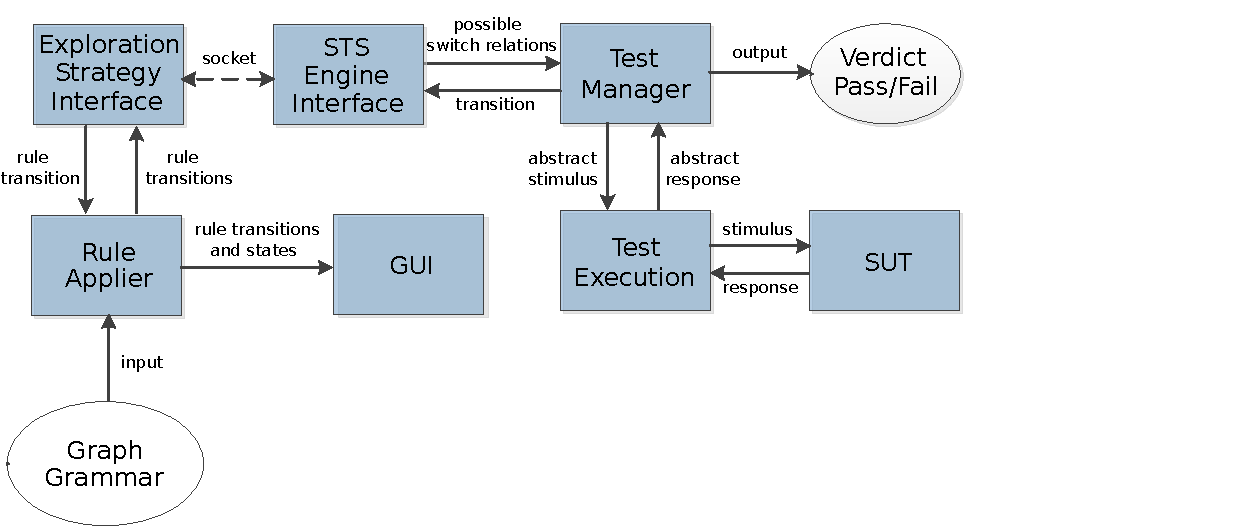
\includegraphics[width=\textwidth]{tooling.pdf}
  \end{center}
  \caption{The GRATiS design: replacing the STS with GROOVE}
  \label{fig:tooling}
\end{figure}

\subsection{Control program}
GROOVE requires variable nodes to be connected to other nodes. This prevents the tool from crashing when a rule contains an unconstrained integer, real or string node. Interaction variables used in responses are often an unknown value coming from the SUT. To model this, a \textit{control program} is needed. This program regulates which rules are applied and chooses values for variables. Figure~\ref{fig:control_program} shows an example of a control program. Here $alap$ lets the program run as long as new graphs are explored. The rule $\ggrule$ is applied or any other rule. $n$ is the image of a variable node marked $parin\colon 0$ when the rule has a match. This node does not need to be connected to other nodes. Using the point algebra, any value can be used for $n \in \mathbb{U}^\sort$, as long as $\sort \in \Sorts$ is the sort of the variable node. This example shows how a variable node can be used to model a response value from the SUT.

\begin{figure}[ht]
  \begin{center}
$\mathit{alap} \{\ggrule(n) | \mathit{other}\}$
  \end{center}
  \caption{A control program}
  \label{fig:control_program}
\end{figure}

\subsection{Rule priority}
There can be several outgoing rule transitions from a graph. However, GROOVE can set different priority levels on rules. A rule transition with a higher priority rule is explored before rule transitions with lower priority rules. Consider the graph grammar in Figure~\ref{fig:priority_gg}. The 'add' rule produces a rule transition to a graph, where the 'sub' rule produces a rule transition back to the start graph. The 'sub' rule does not match the start graph, because it has a lower priority than the 'add' rule.

\begin{figure}[ht]
  \begin{center}
    \subfloat[The start graph state]{\label{fig:priority_start}$\xymatrix{
   \bullet \ar@(dl,dr)[]_{x} \ar[r]^{value} & \bullet \ar@(dl,dr)[]_{0}
}$
}\hspace{20px}
    \subfloat[The LHS of rule 'sub' with priority 1]{\label{fig:priority_lhs1}$\xymatrix{
   \bullet \ar@(dl,dr)[]_{x} \ar[r]^{value} & \bullet \ar[d]^{>} \\
   & \bullet \ar@(dl,dr)[]_{10}
}$
}\hspace{20px}
    \subfloat[The RHS of rule 'sub' with priority 1]{\label{fig:priority_rhs1}$\xymatrix{
   \bullet \ar@(dl,dr)[]_{x} \ar[r]^{value} & \bullet \ar[d]^{-} \\
   & \bullet \ar@(dl,dr)[]_{10}
}$
}\hspace{20px}
    \subfloat[The LHS of rule 'add' with priority 2]{\label{fig:priority_lhs2}$\xymatrix{
   \bullet \ar@(dl,dr)[]_{x} \ar[r]^{value} & \bullet \ar[d]^{<} \\
   & \bullet \ar@(dl,dr)[]_{30}
}$
}\hspace{20px}
    \subfloat[The RHS of rule 'add' with priority 2]{\label{fig:priority_rhs2}$\xymatrix{
   \bullet \ar@(dl,dr)[]_{x} \ar[r]^{value} & \bullet \ar[d]^{+} \\
   & \bullet \ar@(dl,dr)[]_{10}
}$
}
  \end{center}
  \caption{A control node and program in GROOVE}
  \label{fig:priority_gg}
\end{figure} 

The graphs are isomophic under the point algebra, so they represent the same location. The STS of transforming this graph grammar is in Figure~\ref{fig:priority_sts_wrong}, with $\imath = \{x \mapsto 25\}$. This STS is wrong, because the 'sub' switch relation can be taken from the start.

\begin{figure}[ht]
  \begin{center}
    $\xymatrix{
   \ovalbox{$l_0$} \ar@(ul,ur)[]^{?sub\,|\,x\,>\,10\,|\,x\,:=\,x\,-\,10} \ar@(dl,dr)[]_{?add\,|\,x\,<\,30\,|\,x\,:=\,x\,+\,10}
}$

  \end{center}
  \caption{A wrong STS transformation of the graph grammar in Figure~\ref{fig:priority_gg}}
  \label{fig:priority_sts_wrong}
\end{figure}

The solution is shown in Figure~\ref{fig:priority_sts_right}. The negated guard of the 'add' switch relation is added to the 'sub' switch relation. The optimized guard for this switch relation is 'x >= 30' of course, but this shows the main principle: for each outgoing switch relation, the negated guard of all switch relations represented by higher priority rules must be added to the guard. So, the 'x < 30' guard is negated to '!(x < 30)' and added to yield the 'x > 10 \&\& !(x < 30)' guard. Note that if the 'add' switch relation had no guard, it would be applicable on all graph states with isomorphic abstractions. Therefore, the 'sub' switch relation would not exist, because the 'add' rule is always applicable whenever the 'sub' rule also is.

\begin{figure}[ht]
  \begin{center}
    $\xymatrix{
   \fbox{$l_0$} \ar@(ul,ur)[]_{sub | x > 10 \&\& !(x < 30) | x := x - 10} \ar@(dl,dr)[]_{add | x < 30 | x := x + 10}
}$

  \end{center}
  \caption{A correct STS transformation of the graph grammar in Figure~\ref{fig:priority_gg}}
  \label{fig:priority_sts_right}
\end{figure}
